\documentclass[10pt]{beamer}

\usetheme{CambridgeUS}
% Packages
\usepackage[T1]{fontenc}
\usepackage[utf8]{inputenc}
\usepackage[french]{babel}
\usepackage{amsmath}
\usepackage{amssymb}
\usepackage{graphicx}
\usepackage{hyperref}

% Title Information
\title{Prédiction conforme}
\author{H. Hamouda, M. Megdiche}
\institute{Institut National des Sciences Appliquées de Toulouse \\ 3MIC-MA}
\date{\today}

\begin{document}


% Title slide
\begin{frame}
  \titlepage
  \vspace{1cm}
  {\small \centering Encadré par: Prof. Joseba Dalmau \par}
\end{frame}




% Résultat de la prédiction conforme
\begin{frame}{Résultat de la prédiction conforme}
\small
\begin{block}{Théorème}
Soit, pour $i = 1, \ldots, n$,
\[
(X_i, Y_i) \sim P_{\mathcal{X}\mathcal{Y}}
\]
une suite de couples de variables aléatoires, indépendantes et identiquement distribuées. Les $(X_i, Y_i)$ prennent leurs valeurs dans $\mathcal{X} \times \mathcal{Y}$. On définit également $\alpha$, le niveau d'erreur pour notre prédiction.

On construit $\hat{C}$ telle que :
\[
\hat{C} : \mathcal{X} \to \mathcal{P}(\mathcal{Y})
\]
où $\mathcal{P}(\mathcal{Y})$ désigne l'ensemble des parties de $\mathcal{Y}$.

Cette fonction a pour propriété que, pour une nouvelle paire de test $(X_{\text{test}}, Y_{\text{test}}) \sim P_{\mathcal{X}\mathcal{Y}}$,
\[
\hat{C}(X_{\text{test}}) = \left\{ y \in \mathcal{Y} \mid s(X_{\text{test}}, y) < q \right\}
\]
où $s$ est une fonction de score et $q$ un seuil défini ci-dessous.

On a donc :
\[
\mathbb{P}\left( Y_{\text{test}} \in \hat{C}(X_{\text{test}}) \right) \geq 1 - \alpha
\]
\end{block}
\end{frame}

% Slide: suite du Résultat de la prédiction conforme
\begin{frame}{Résultat de la prédiction conforme}
\begin{block}{suite}
les scores de calibration sont tels que:
\begin{itemize}
    \item $s_1 = s(X_1, Y_1), \ldots, s_n = s(X_n, Y_n)$
    \item $q$ est le $\lceil (n+1)(1-\alpha) \rceil$-quantile de la suite $(s_1, \ldots, s_n)$
\end{itemize}
\end{block}
\end{frame}

% 2 Slides: Applications du théorème de la prédiction conforme
% application sur la régression linéaire

\begin{frame}{Applications du théorème de la prédiction conforme}
\small
Problème de regression linéaire:
    Soit\\
    \begin{itemize} 
    \item $(X_1, Y_1), \dots, (X_n, Y_n)$ i.i.d. sur $\mathcal{X} \times \mathbb{R}$ un ensemble de calibration
    \item $(X_{\text{test}}, Y_{\text{test}})$ un point test indépendant issu de la même distribution.\\
    
    \item $\hat{f} : \mathcal{X} \to \mathbb{R}$ un modèle de régression linéaire entraîné sur un autre jeu de données\\
    on a donc dans ce cas:
    \begin{itemize}
        \item Les scores de non-conformité : $s_i = |Y_i - \hat{f}(X_i)|$ pour $i = 1, \dots, n$ ;
        \item Le quantile empirique conforme :
        \[
        \hat{q} = \text{score au rang } \left\lceil (n+1)(1 - \alpha) \right\rceil \text{ parmi les } s_i ;
        \]
        \item L'ensemble prédictif conforme :
        \[
        \hat{C}_n(x) = \left[ \hat{f}(x) - \hat{q},\; \hat{f}(x) + \hat{q} \right] .
        \] est continu
    \end{itemize}
    \end{itemize}
    Alors, l'ensemble $\hat{C}_n(x)$ satisfait la propriété:
    \[
    \mathbb{P}\left( Y_{\text{test}} \in \hat{C}_n(X_{\text{test}}) \right) \geq 1 - \alpha
    \]
    où la probabilité est prise conjointement sur les données de calibration et le point test.

\end{frame}

\begin{frame}{visualisation}
    \centering
    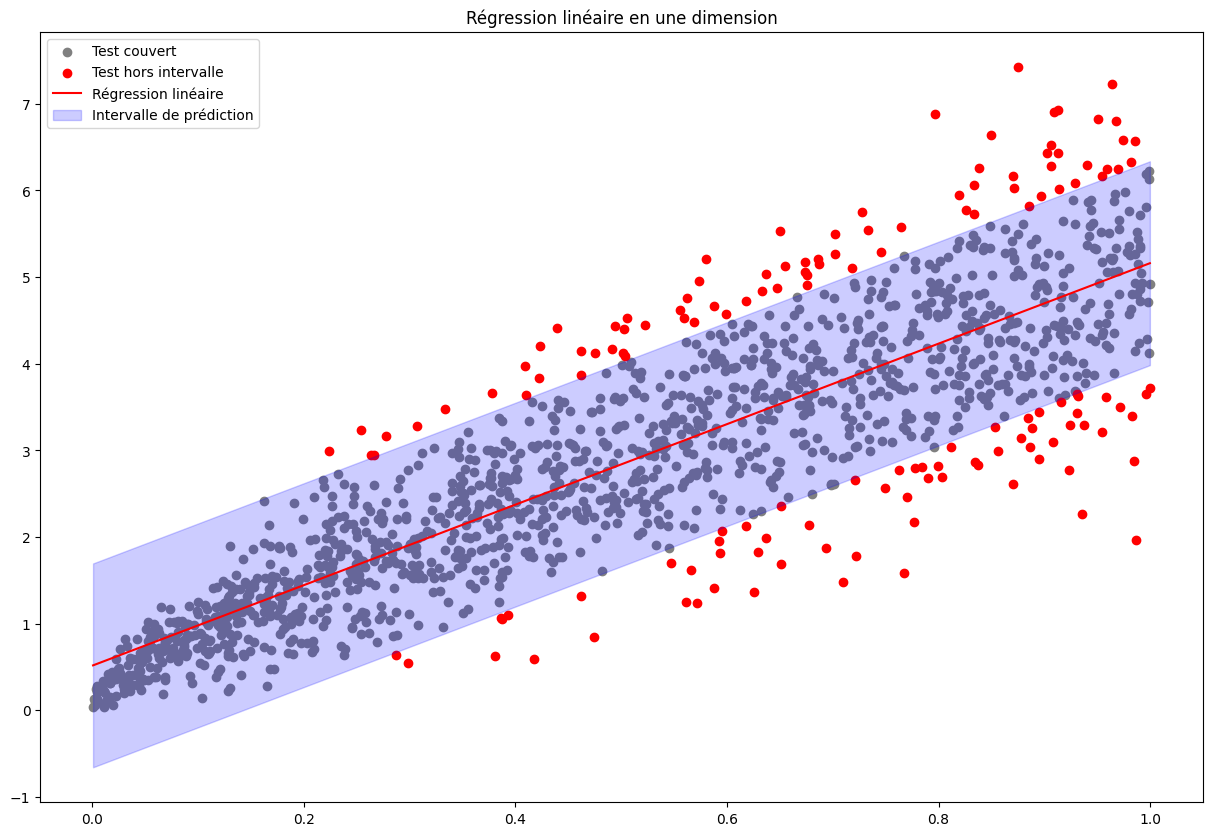
\includegraphics[width=0.7\textwidth]{conformal_prediction_regression.png}

    \vspace{0.5em}
    \small
    \textit{prédiction conforme sur des données de test $(X_i,Y_i)_{0 \dots 149},$ au niveau $\alpha= 1\% $}
\end{frame}
\end{frame}



\begin{frame}{Applications du théorème de la prédiction conforme}
\small
   Problème de classification:
   on a $\mathcal{Y} = \{1, \dots, K\}$ un ensemble fini de classes.
        \begin{itemize}
        \item $\{(X_1, Y_1), \dots, (X_n, Y_n)\}$ paires i.i.d. de distribution inconnue sur $\mathcal{X} \times \mathcal{Y}$, ensemble de calibration, $(X_{\text{test}}, Y_{\text{test}})$ une paire test indépendante et $(X_{\text{test}}, Y_{\text{test}}) \sim P_{\mathcal{X}\mathcal{Y}}$.
        
        \item $\hat{f} : \mathcal{X} \rightarrow \Delta_K$ un modèle de classification MNIST entraîné, où $\Delta_K$ est le simplexe de dimension $K-1$ (i.e. l'ensemble des vecteurs de probabilités de classe).\\
        On note $\hat{f}(x) = (p_1(x), \dots, p_K(x))$ les probabilités prédites pour chaque classe.
        
        Définissons :
        \begin{itemize}
            \item Le score de non-conformité pour chaque point de calibration :
            \[
            s_i = 1 - \hat{f}_{Y_i}(X_i), \quad \text{pour } i = 1, \dots, n,
            \]
            où $\hat{f}_{Y_i}(X_i)$ est la probabilité attribuée par le modèle à la vraie classe $Y_i$.
           
            \item Le seuil conforme comme le quantile empirique :
            \[
            \hat{q} = \text{score au rang } \left\lceil (n+1)(1 - \alpha) \right\rceil \text{ parmi les } \{s_i\}_{i=1}^n.
            \]
           
            \item L'ensemble de prédiction conforme :
            \[
            \hat{C}_n(x) = \left\{ y \in \mathcal{Y} : 1 - \hat{f}_y(x) \leq \hat{q} \right\}.
            \]
        \end{itemize}
        \end{itemize}
        Alors, sous l'hypothèse d'échangeabilité des $n+1$ exemples, on a la garantie suivante :
        \[
        \mathbb{P}\left( Y_{\text{test}} \in \hat{C}_n(X_{\text{test}}) \right) \geq 1 - \alpha,
        \]
        où la probabilité est prise sur les données de calibration et le point test.
\end{frame}

% Slide: Document minimal
\begin{frame}[fragile]{Document minimal}
\begin{verbatim}
\documentclass{article}
\begin{document}
Tout ce que je veux afficher dans mon document
\end{document}
\end{verbatim}
\end{frame}

% Slide: Mathématiques
\begin{frame}{Mathématiques}
\begin{block}{Modes mathématiques}
\begin{itemize}
    \item En ligne : \texttt{\$...\$} ou \texttt{\(...\)}
    \item Centré : \texttt{\[...\]} ou \texttt{\$\$...\$\$}
\end{itemize}
\end{block}

\begin{block}{Exemple}
Soit $x$ une variable réelle solution de l’équation :
\[
ax^2 + bx + c = 0
\]
Le discriminant vaut $\Delta = b^2 - 4ac$. S’il est strictement positif, il y a deux racines réelles distinctes :
\[
x_1 = \frac{-b - \sqrt{\Delta}}{2a}, \quad x_2 = \frac{-b + \sqrt{\Delta}}{2a}
\]
\end{block}
\end{frame}

% Slide: Exercices avancés
\begin{frame}{Exercices avancés}
\begin{enumerate}
    \item Navier-Stokes :
    \[
    \frac{\partial \vec{v}}{\partial t} + \left( \vec{v} \cdot \nabla \right) \vec{v} = -\frac{1}{\rho} \nabla p + \nu \nabla^2 \vec{v} + \vec{f}
    \]
    \item Lotka-Volterra :
    \[
    \frac{dx}{dt} = x(\alpha - \beta y), \quad \frac{dy}{dt} = -y(\gamma - \delta x)
    \]
    \item Intégrale gaussienne :
    \[
    \delta \int_{0}^{\infty} \int_{0}^{\infty} e^{-(x^2 + y^2)} \, dx \, dy = \frac{\pi}{4}
    \]
\end{enumerate}
\end{frame}

% Slide: Bibliographie
\begin{frame}[fragile]{Bibliographie}
Exemple de fichier \texttt{.bib}:
\begin{verbatim}
@BOOK{HofbSigm98,
title = {Evolutionary Games and Population Dynamics},
publisher = {Cambridge University Press},
year = {1998},
author = {Joseph Hofbauer, Karl Sigmund}
}
\end{verbatim}
\end{frame}

% Slide: Conclusion
\begin{frame}{Conclusion}
Pour aller plus loin : \url{http://www.jalix.org/ressources/miscellaneous/tex/_faq-latex2/html/}
\end{frame}

\end{document}
